\chapter*{Appendix: Tables and Figures}
\addcontentsline{toc}{chapter}{Appendix: Tables and Figures}
\section*{1 Tables}
\addcontentsline{toc}{section}{Tables}

\begin{table}[h!]
\centering
\begin{tabular}{lcccc}
\toprule
\textbf{Factor} & $\mu$ (in \%, annual) & $\sigma$ (in \%, annual) & Max (in \%) & Min (in \%) \\
\midrule
MKT & 7.078 & 16.185 & 11.3 & -17.4 \\
SMB & 1.592 & 8.740 & 6.2 & -11.2 \\
HML & 3.466 & 9.300 & 6.7 & -5.0 \\
RMW & 3.482 & 6.376 & 4.5 & -3.0 \\
CMA & 3.040 & 6.041 & 2.5 & -5.9 \\
\bottomrule
\end{tabular}
\caption{Summary statistics of factor returns. $\mu$ and $\sigma$ are annualized.}
\label{tab:factor_stats}
\end{table}

\begin{table}[htbp]
\centering
\caption{Sharpe ratios and Ledoit–Wolf tests (OOS, 1963–2024)}
\label{tab:sr_main}
\setlength{\tabcolsep}{6pt}
\renewcommand{\arraystretch}{1.15}
\begin{tabular}{lccccc}
\toprule
& MKT & SMB & HML & RMW & CMA \\
\midrule
\multicolumn{6}{l}{\emph{Sharpe ratios}}\\
SR: Original    & 0.397 & -0.256 & 0.259 & 0.178 & 0.242 \\
SR: Vol-Managed & 0.513 & -0.225 & 0.393 & 0.306 & 0.127 \\
SR: EPU-Managed & 0.515 & -0.236 & 0.307 & 0.236 & 0.197 \\
\midrule
$\Delta SR$ (Vol$-$Orig) & \valp{0.116}{0.969} & \valp{0.031}{0.977} & \valp{0.134}{0.965} & \valp{0.127}{0.980} & \valp{-0.115}{0.977} \\
$\Delta SR$ (EPU$-$Orig) & \valp{0.118}{0.940} & \valp{0.020}{0.982} & \valp{0.049}{0.998} & \valp{0.057}{0.950} & \valp{-0.045}{0.974} \\
$\Delta SR$ (EPU$-$Vol)  & \valp{0.002}{0.992} & \valp{-0.011}{0.982} & \valp{-0.085}{0.970} & \valp{-0.070}{0.950} & \valp{0.070}{0.965} \\
\bottomrule
\end{tabular}

\medskip
\footnotesize Notes: SRs are annualized. Differences tested with Ledoit–Wolf $Z$-test using 6-month block bootstrap with 10{,}000 repetitions. P-values in parentheses.
\end{table}

\begin{table}[htbp]
\centering
\caption{Alpha tests: managed vs. original factor (monthly OLS, NW $L\!=\!6$)}
\label{tab:alpha_main}
\setlength{\tabcolsep}{6pt}
\renewcommand{\arraystretch}{1.15}
\begin{tabular}{lccccc}
\toprule
& MKT & SMB & HML & RMW & CMA \\
\midrule
\multicolumn{6}{l}{\emph{Volatility-managed vs. Original}}\\
$\alpha$         & \valp{0.0032}{0.480} & \valp{-0.0018}{0.375} & \valp{0.0005}{0.816} & \valp{0.0000}{0.980} & \valp{0.0023}{0.131} \\
$R^2$            & 0.385 & 0.581 & 0.355 & 0.332 & 0.385 \\
RMSE             & 0.0091 & 0.0040 & 0.0048 & 0.0038 & 0.0032 \\
\midrule
\multicolumn{6}{l}{\emph{EPU-managed vs. Original}}\\
$\alpha$         & \valp{0.0059}{0.135} & \valp{-0.0013}{0.452} & \valp{0.0011}{0.540} & \valp{0.0009}{0.493} & \valp{0.0016}{0.300} \\
$R^2$            & 0.472 & 0.558 & 0.396 & 0.324 & 0.368 \\
RMSE             & 0.0076 & 0.0038 & 0.0042 & 0.0036 & 0.0031 \\
\bottomrule
\end{tabular}

\medskip
\footnotesize Notes: $\alpha$ in monthly units. Newey–West standard errors with 6 lags. P-values in parentheses. Sample size $N = 617$ months.
\end{table}

\clearpage
\section*{2 Figures}
\addcontentsline{toc}{section}{Figures}

\begin{figure}[h]
  \centering
  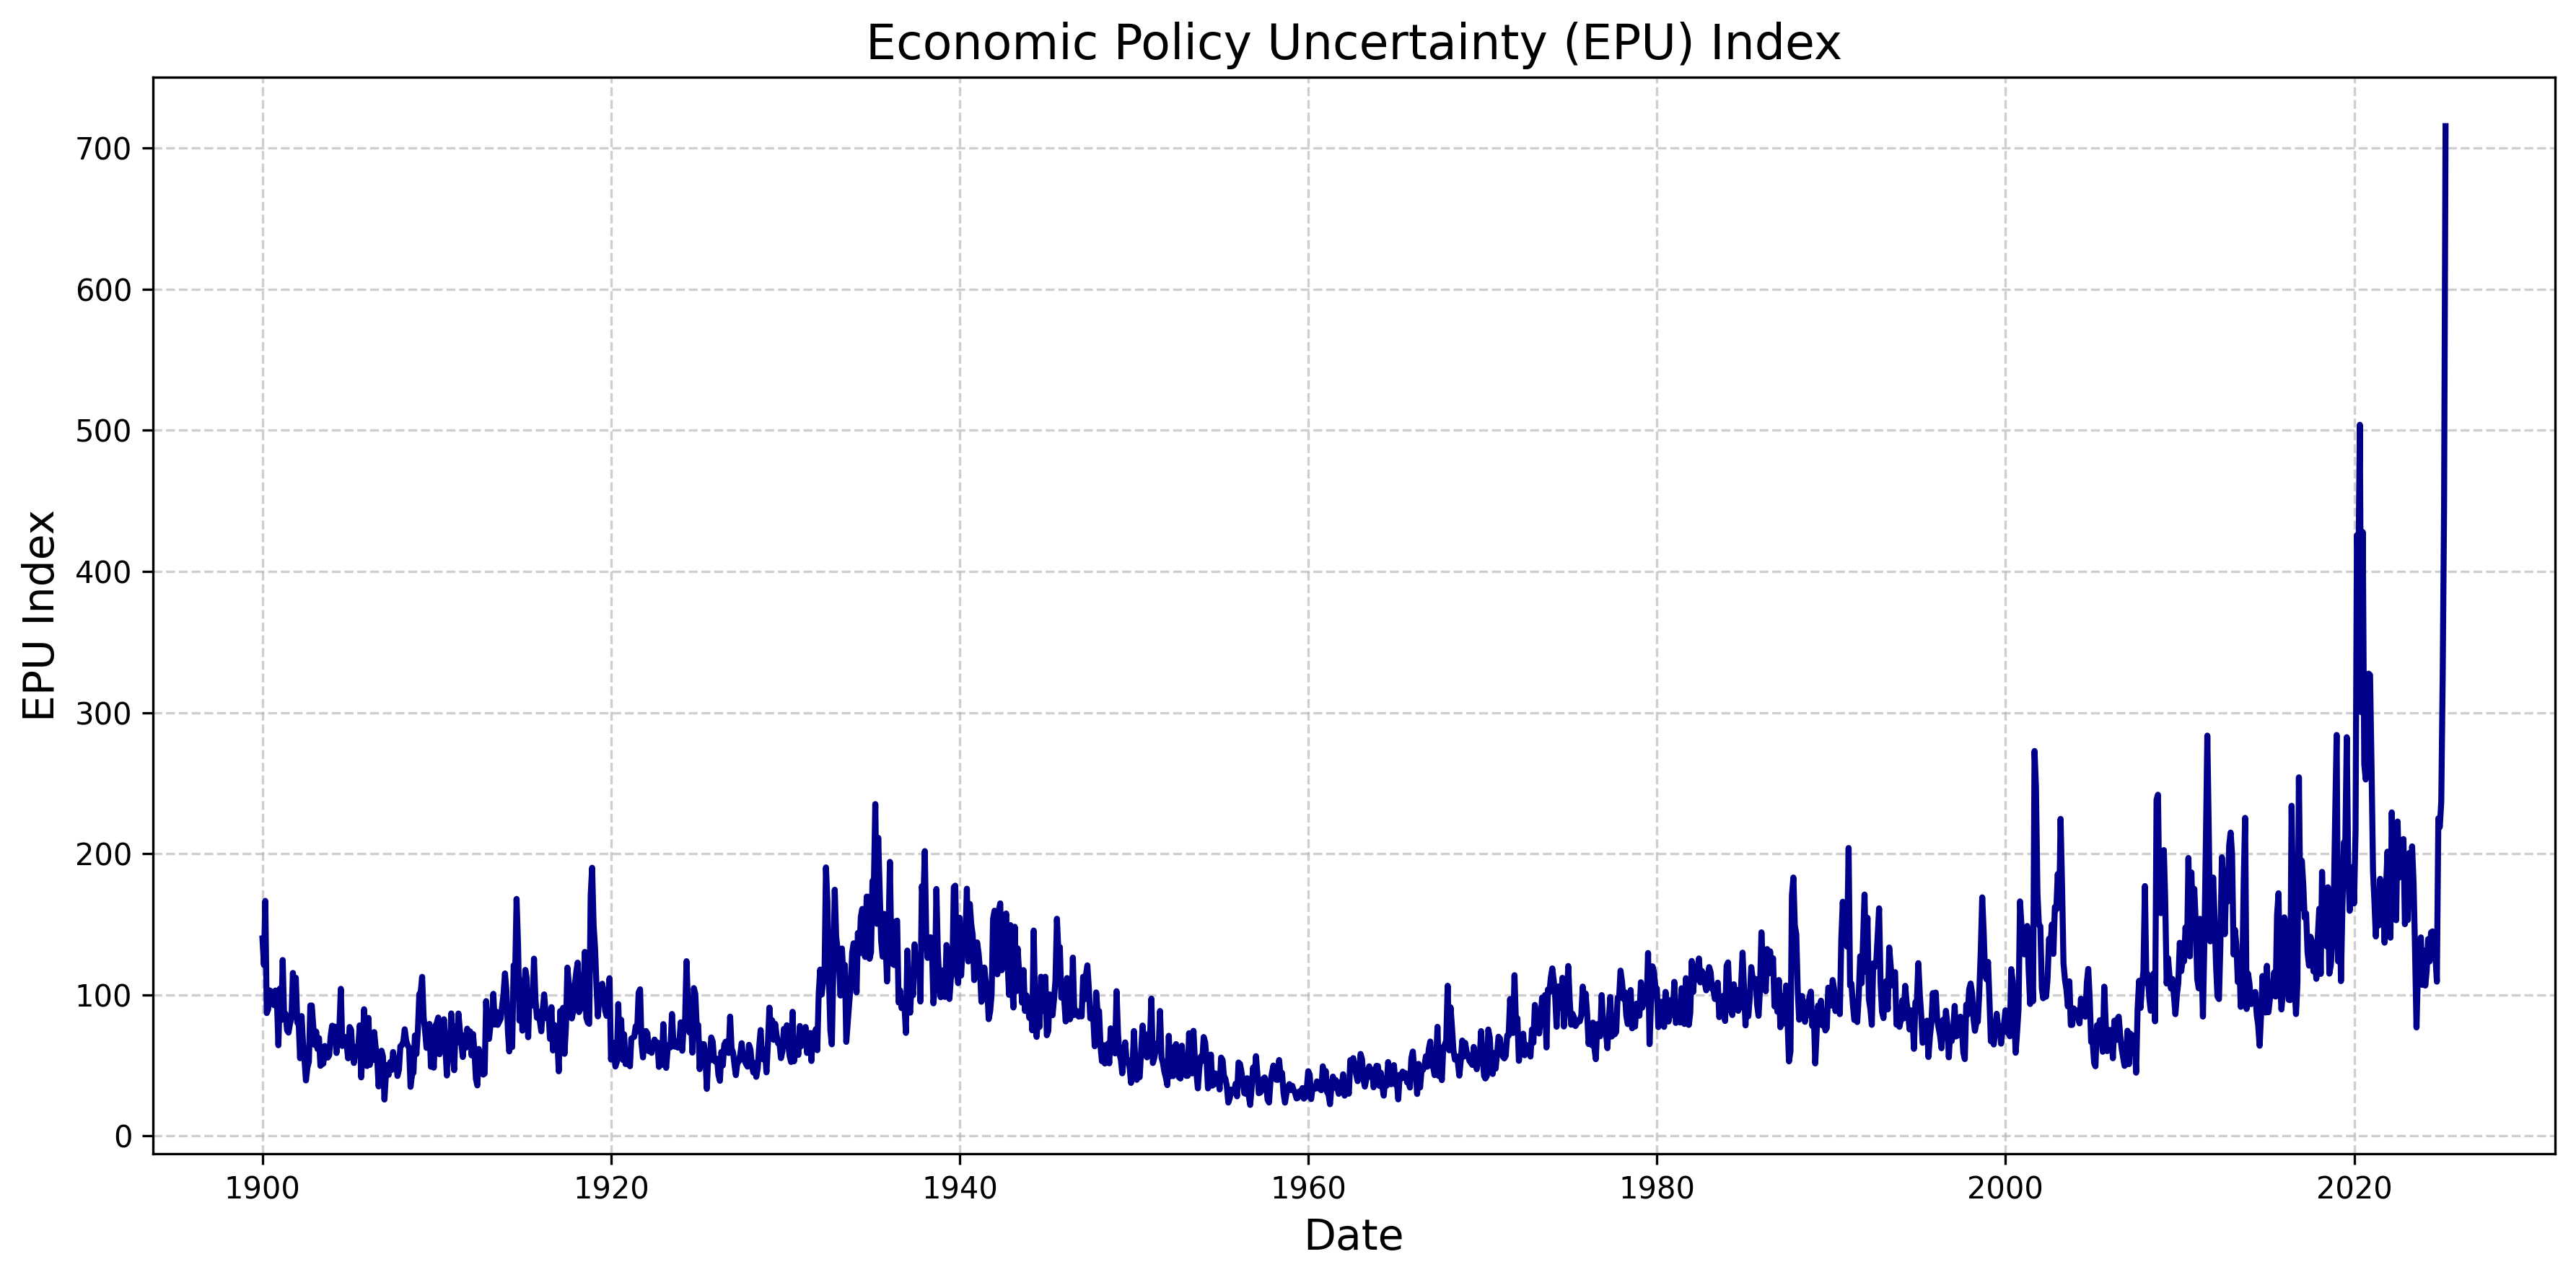
\includegraphics[width=1\linewidth]{Images/EPU_indicator_US.png}
  \caption{Economic Policy Uncertainty (EPU) index}
  \label{fig:EPU}
\end{figure}

\begin{figure}[h]
  \centering
  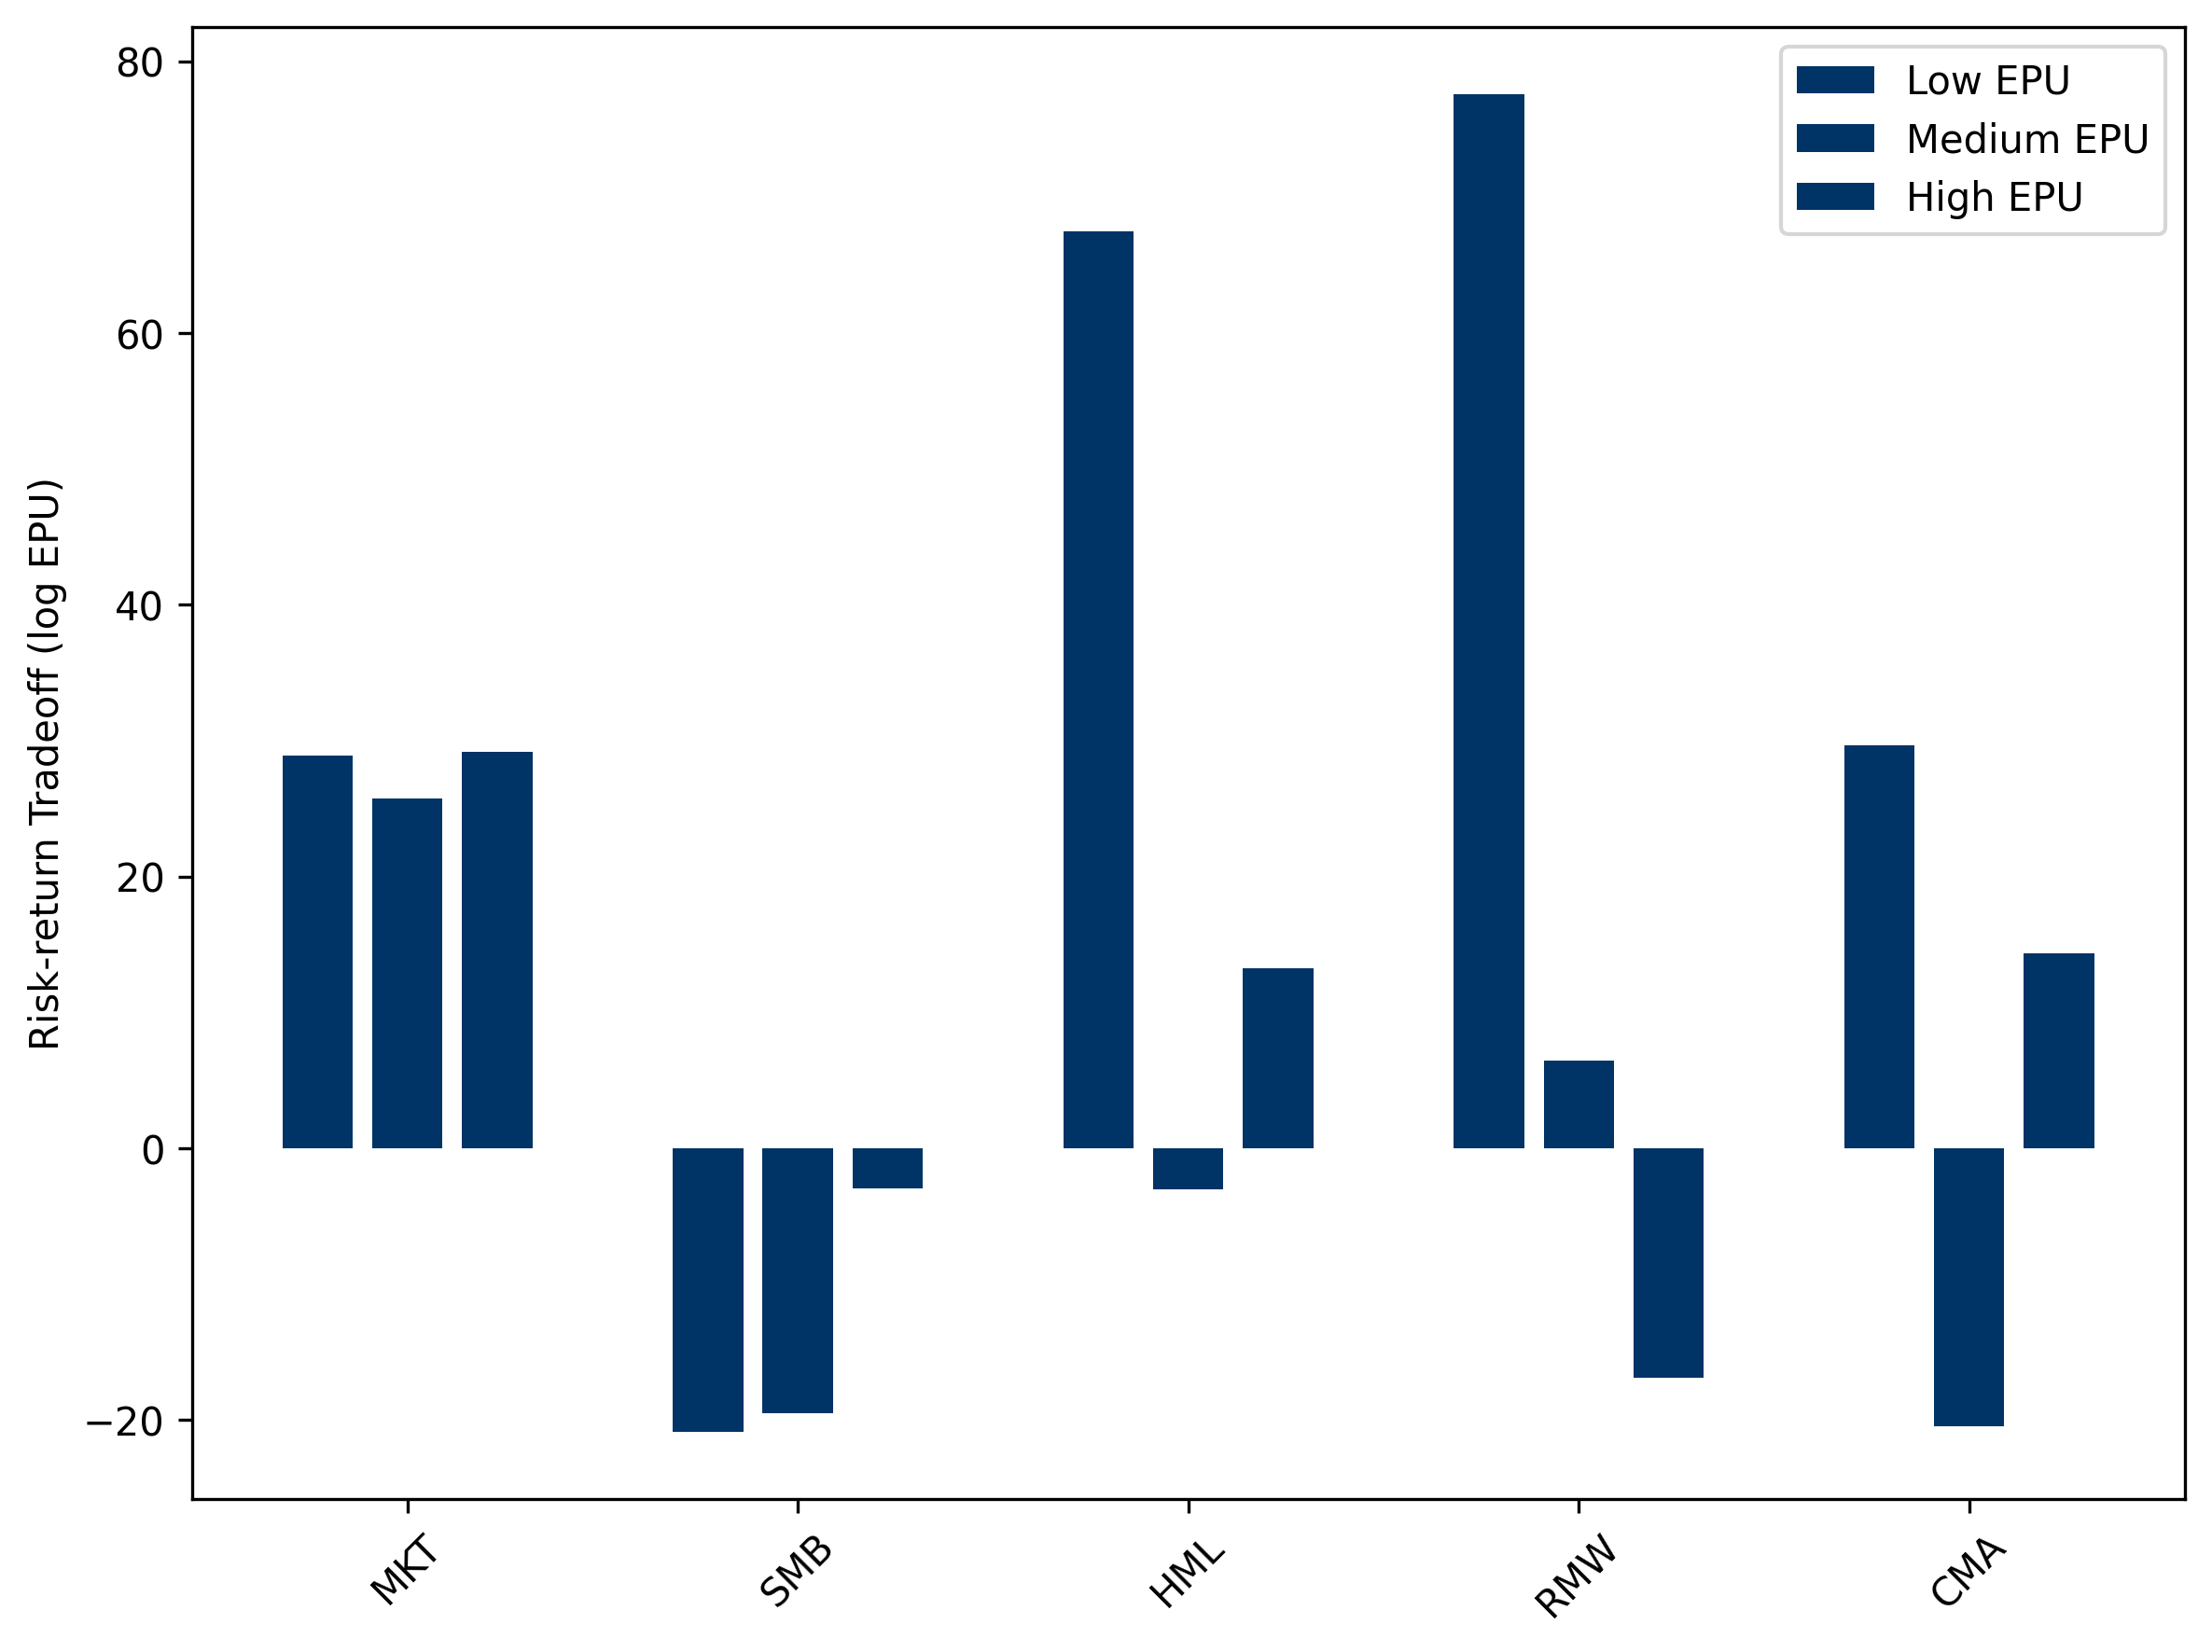
\includegraphics[width=1\linewidth]{Images/EPU-based buckets.png}
  \caption{EPU-based buckets}
  \label{fig:EPU-based buckets}
\end{figure}

\begin{figure}[h]
  \centering
  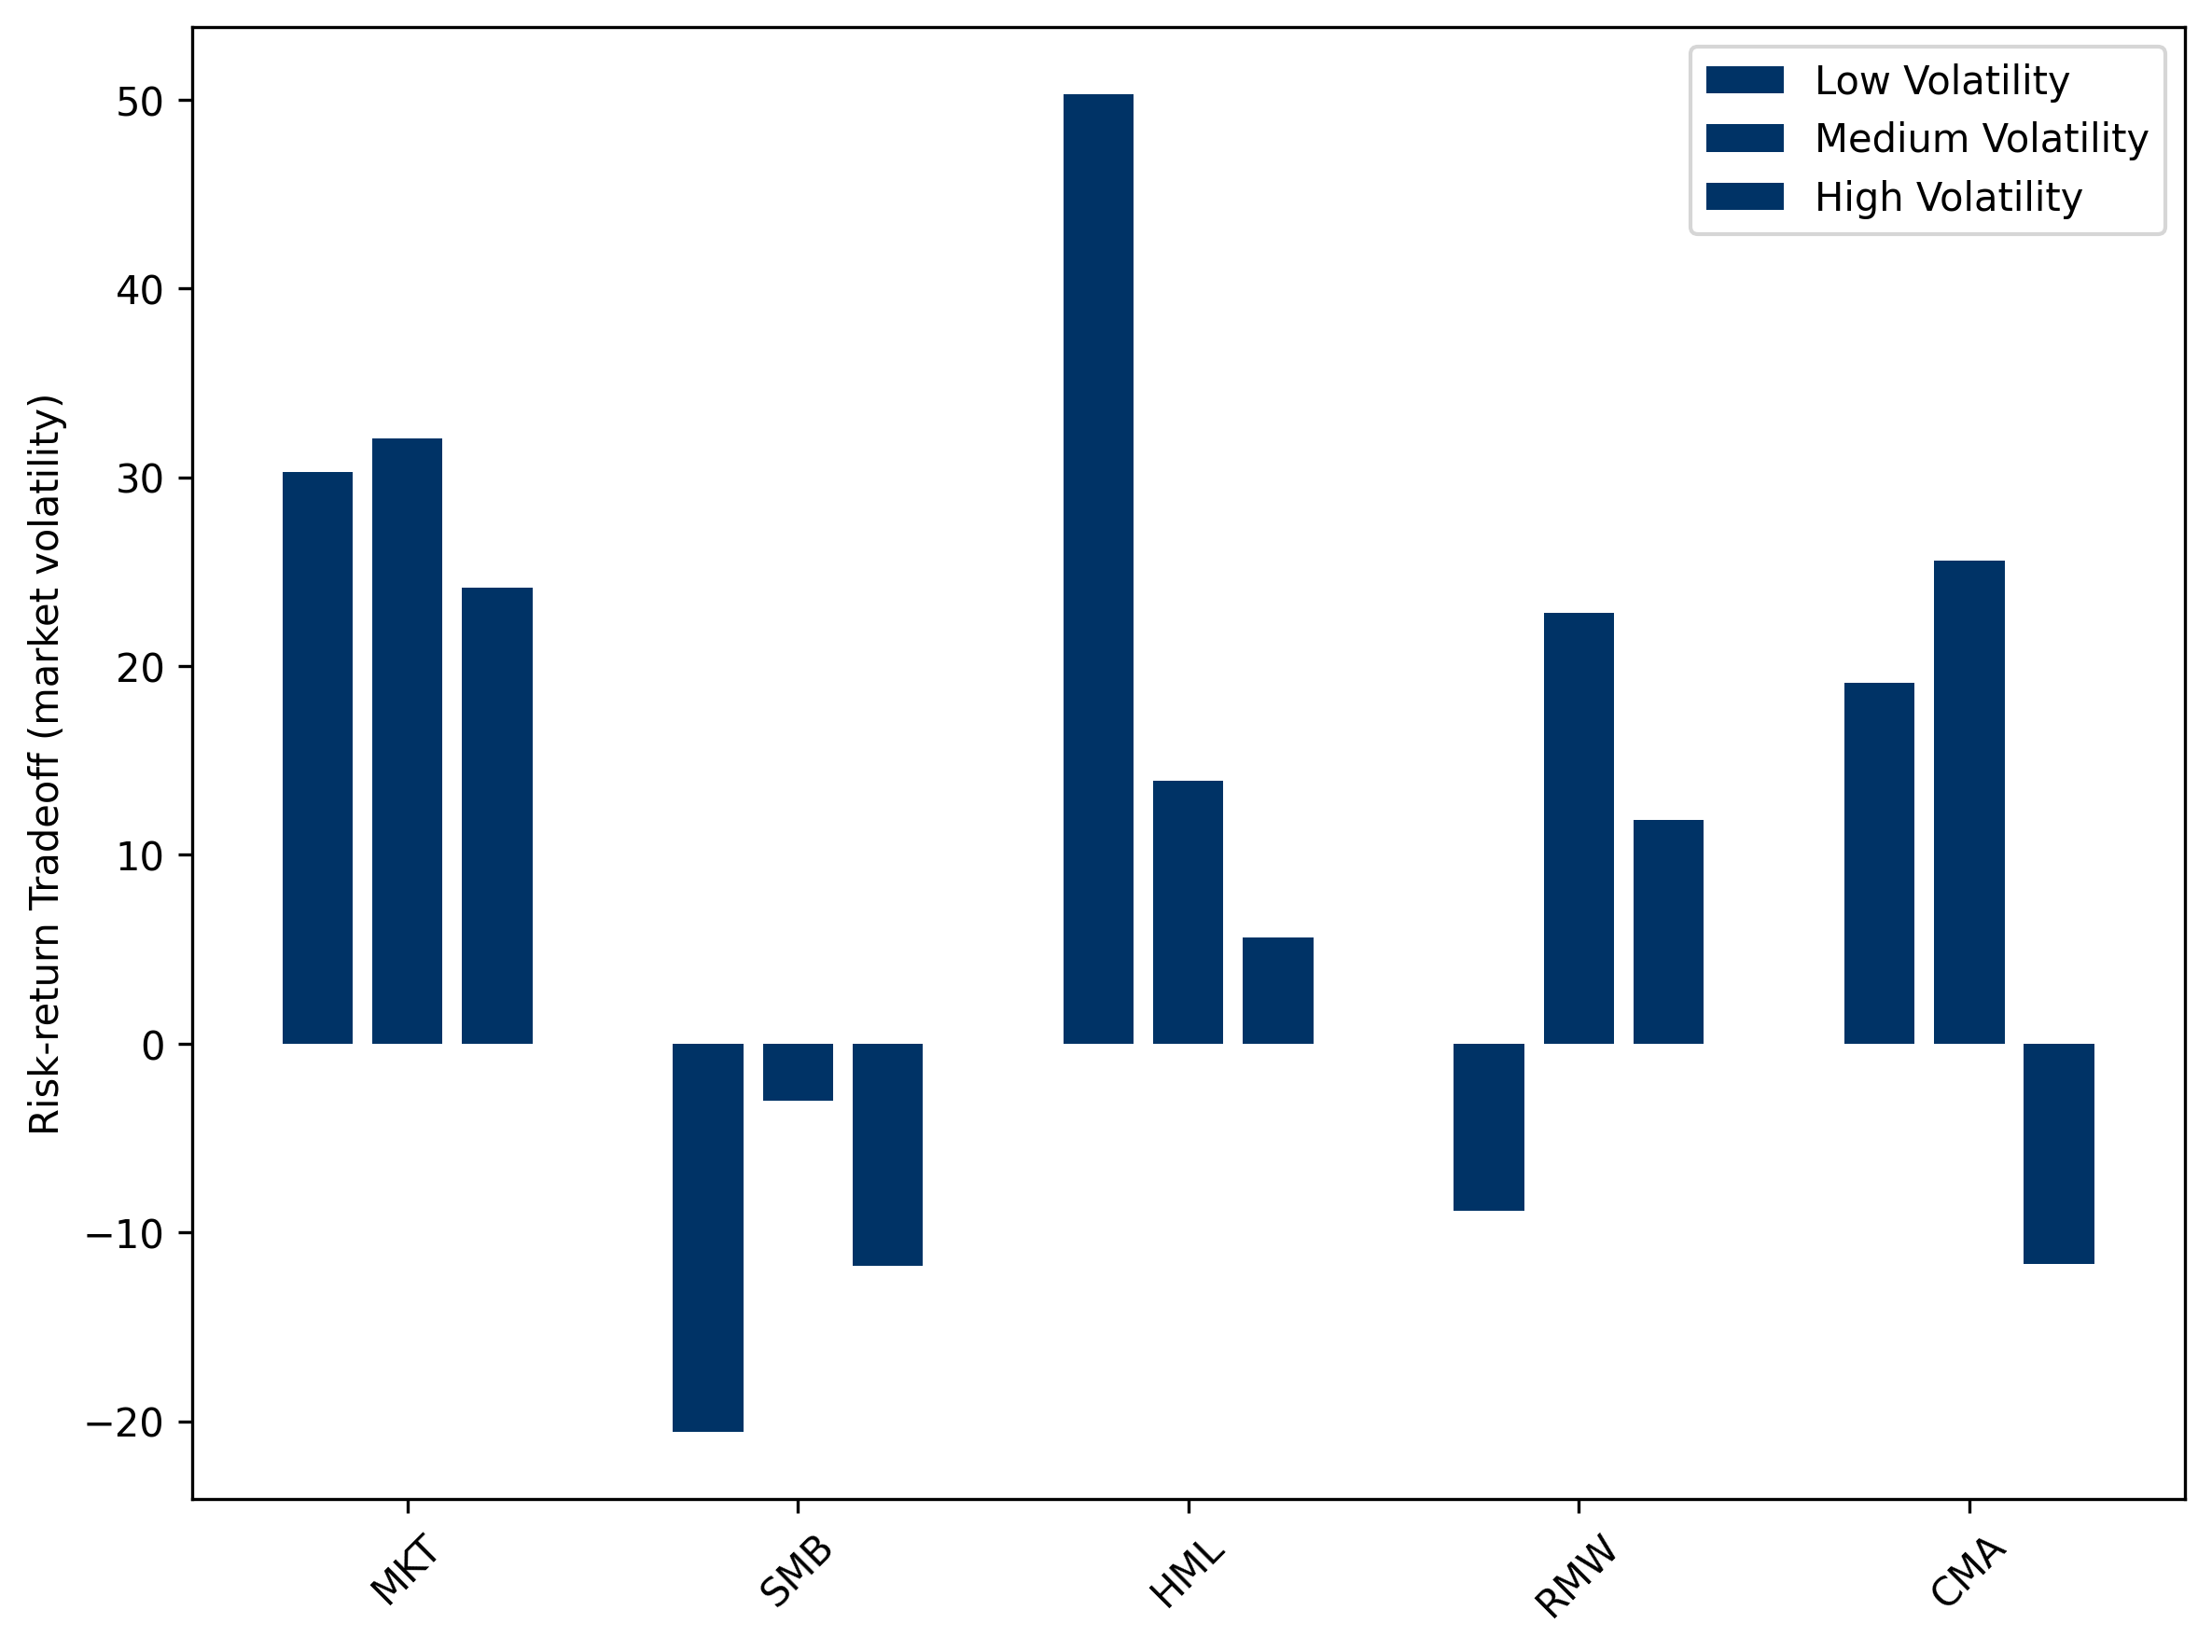
\includegraphics[width=1\linewidth]{Images/Volatility-based buckets.png}
  \caption{Volatility-based buckets}
  \label{fig:Volatility-based buckets}
\end{figure}
